\documentclass{scrreprt}

\usepackage{aligned-overset}
\usepackage{amsmath}
\usepackage{amsthm}
\usepackage{amssymb}
\usepackage{bm}
\usepackage[inline,shortlabels]{enumitem}
\usepackage{hyperref}
\usepackage[utf8]{inputenc}
\usepackage{multicol}
\usepackage{mathtools}
\usepackage{pdflscape}
\usepackage{physics}
\usepackage{tabularx}
\usepackage[table]{xcolor}
\usepackage{titling}
\usepackage{fancyhdr}
\usepackage{xfrac}
\usepackage{pgfplots}

\pgfplotsset{compat = newest}
\usepgfplotslibrary{fillbetween}
\usetikzlibrary{calc}


\author{Karsten Lehmann}
\date{SoSe 2025}
\title{Übungsblatt 01\\INF-B-120, Mathematische Methoden für Informatiker}

\setlength{\parindent}{0pt}

\setlength{\headheight}{26pt}
\pagestyle{fancy}
\fancyhf{}
\lhead{\thetitle}
\rhead{\theauthor}
\lfoot{\thedate}
\rfoot{Seite \thepage}

\begin{document}
\paragraph{Ü 1.1}
\begin{enumerate}[(a)]
\item Die Zeichnung zeigt eine Folge von vier Figuren.
  Man stelle sich vor, dass die Zerlegung in dieser Form weitergeführt wird.
  Es bezeichne $x_n$ die Anzahl der quadratischen Teile, aus denen die $n$-te
  Figur besteht.
  Finden Sie eine rekursive und eine explizite Formel für $x_n$.

  \begin{minipage}{.15\textwidth}
    \begin{tikzpicture}
      \draw (0, 0) -- (2, 0) -- (2, 2) -- (0, 2) -- (0, 0);
    \end{tikzpicture}
  \end{minipage}
  \begin{minipage}{.15\textwidth}
    \begin{tikzpicture}
      \draw (0, 0) -- (2, 0) -- (2, 2) -- (0, 2) -- (0, 0);
      \draw (1, 0) -- (1, 2);
      \draw (0, 1) -- (2, 1);
    \end{tikzpicture}
  \end{minipage}
  \begin{minipage}{.15\textwidth}
    \begin{tikzpicture}
      \draw (0, 0) -- (2, 0) -- (2, 2) -- (0, 2) -- (0, 0);
      \draw (1, 0) -- (1, 2);
      \draw (0, 1) -- (2, 1);
      \draw (1, 1.5) -- (2, 1.5);
      \draw (1.5, 1) -- (1.5, 2);
    \end{tikzpicture}
  \end{minipage}
  \begin{minipage}{.15\textwidth}
    \begin{tikzpicture}
      \draw (0, 0) -- (2, 0) -- (2, 2) -- (0, 2) -- (0, 0);
      \draw (1, 0) -- (1, 2);
      \draw (0, 1) -- (2, 1);
      \draw (1, 1.5) -- (2, 1.5);
      \draw (1.5, 1) -- (1.5, 2);
      \draw (1.75, 2) -- (1.75, 1.5);
      \draw (1.5, 1.75) -- (2, 1.75);
    \end{tikzpicture}
  \end{minipage}

  \subparagraph{Lsg.} \underline{Variante 1:} Wir zählen nur die inneren
  Quadrate, somit hat die Folge $x_n$ die ersten Glieder $1, 4, 7, 10$.
  Dabei ist $x_{n + 1} \coloneqq x_n + 3$ und $x_n \coloneqq 3n - 2$.

  \underline{Variante 2:} Wir zählen alle Quadrate, somit hat die Folge $y_n$ die
  ersten Glieder $1, 5, 9, 13$.
  Dabei ist $y_{n + 1} \coloneqq y_n + 4$ und $y_n \coloneqq 4n - 3$.


\item Von der reellen Zahlenfolge $\qty\big(x_n)_{n \in \mathbb{N}}$ ist
  bekannt, dass $x_{100} = 7$ und $x_{402} = 6$ ist und die Summe von je drei
  aufeinanderfolgenden Gliedern der Folge $\qty\big(x_n)$ gleich 10 ist.
  Welchen Wert hat dann $x_{500}$?

  \subparagraph{Lsg.} Für die Folge gilt
  \[
    \forall n \in \mathbb{N} \colon x_n + x_{n + 1} + x_{n + 2} = 10
  \]
  Es folgt
  \[
    \begin{array}{cccccccccc}
        & x_n & + & x_{n + 1} & + & x_{n + 2} &   &          & = & 10 \\
      - &     &   & x_{n + 1} & + & x_{n + 2} & + & x_{n + 3} & = & 10 \\
      \cline{2-10}
        & x_n & - &          &    &          &   & x_{n + 3} & = & 0 \\
    \end{array}
  \]
  $\Rightarrow x_n = x_{n + 3}$
  Schließlich folgt $x_{501} = x_{402} = 6$, da $501 \mod 3 = 402 \mod 3 = 0$
  als auch $x_{502} = x_{100} = 7$, da $502 \mod 3 = 100 \mod 3 = 1$ und
  schlussendlich $x_{500} = 10 - x_{502} - x_{501} = -3$.

\newpage
\item Untersuchen Sie die Folgen $\qty\big(x_n)_{n \in \mathbb{N}}$ darauf,
  ob sie ab einem Index $n_0$ monoton sind:

  \begin{enumerate*}[(1)]
  \item $x_n \coloneqq \frac{2n - 7}{3n - 10}$
  \item $x_n \coloneqq \frac{7n + 1}{3n - 1}$
  \item $x_n \coloneqq \frac{n}{5} + \frac{5}{n}, n > 1$
  \end{enumerate*}

  \subparagraph{Lsg.} Der \emph{``Trick''} dabei ist immer das vorherige
  Folgenglied vom nächsten abzuziehen:
  \begin{enumerate}[(1)]
  \item \begin{flalign*}
      x_{n + 1} - x_n
      &= \frac{2\qty\big(n + 1) - 7}{3\qty\big(n + 1) - 10} - \frac{2n - 7}{3n - 10} & \\
      &= \frac{2n + 2 - 7}{3n + 3 - 10} - \frac{2n - 7}{3n - 10} \\
      &= \frac{2n - 5}{3n - 7} - \frac{2n - 7}{3n - 10} \\
      &= \frac{\qty\big(3n - 10)\qty\big(2n - 5) - \qty\big(2n - 7)\qty\big(3n - 7)}{\qty\big(3n - 7)\qty\big(3n - 10)} \\
      &= \frac{\qty\big(6n^2 - 35n + 50) - \qty\big(6n^2 - 35n + 49)}{\qty\big(3n - 1)\qty\big(3n - 10)} \\
      &= \frac{1}{\qty\big(3n - 1)\qty\big(3n - 10)}
    \end{flalign*}
    und nun zu schauen, für welches $n_0$ gilt, dass für alle $m \in \mathbb{N}$
    mit $m \geq n_0$ sich das Vorzeichen des Ergebnis nicht mehr ändert.
    Nun ist der Term offensichtlich für $n_0 = 4$ immer größer Null und damit die
    Folge ab dem Index $n_0$ streng monoton wachsend.

  \item \begin{flalign*}
      x_{n + 1} - x_n
      &= \frac{7\qty\big(n + 1) + 1}{3\qty\big(n + 1) - 1} - \frac{7n + 1}{3n - 1} & \\
      &= \frac{7n + 7 + 1}{3n + 3 - 1} - \frac{7n + 1}{3n - 1} \\
      &= \frac{7n + 8}{3n + 2} - \frac{7n + 1}{3n - 1} \\
      &= \frac{\qty\big(7n + 8)\qty\big(3n - 1) - \qty\big(7n + 1)\qty\big(3n + 2)}{\qty\big(3n + 2)\qty\big(3n - 1)} \\
      &= \frac{\qty\big(21n^2 + 17n - 8) - \qty\big(21n^2 + 17n + 2)}{\qty\big(3n + 2)\qty\big(3n - 1)} \\
      &= -\frac{6}{\qty\big(3n + 2)\qty\big(3n - 1)}
    \end{flalign*}
    Nun ist der Term ab dem Index $n_0 = 1$ kleiner als 0 und die Folge damit
    streng monoton fallend.

  \item \begin{flalign*}
      x_{n + 1} - x_n
      &= \qty(\frac{n + 1}{5} + \frac{5}{n + 1}) - \qty(\frac{n}{5} + \frac{5}{n}) & \\
      &= \frac{n + 1}{5} + \frac{5}{n + 1} - \frac{n}{5} - \frac{5}{n} \\
      &= \frac{1}{5} + \frac{5n}{n^2 + n} - \frac{5n + 5}{n^2 + n} \\
      &= \frac{1}{5} - \frac{5}{n^2 + n}
    \end{flalign*}
    Nun ist der Term ab dem Index $n_0 = 5$ größer als 0 und die Folge damit
    streng monoton steigend.
  \end{enumerate}
\end{enumerate}

\paragraph{Ü 1.2}
\begin{enumerate}[(a)]
\item Skizzieren Sie den Graph der Wurzelfunktion und betrachten Sie die Folge
  $\qty\big(x_n)_{n \in \mathbb{N} \setminus \qty\big{0}}$ mit
  $x_n \coloneqq \sqrt{\frac{1}{n}}$.
  Welches Monotonieverhalten zeigt $\qty\big(x_n)$?

  \subparagraph{Lsg.} Der Graph:

  \begin{tikzpicture}[scale=1]
    \begin{axis}[
      axis equal,
      axis x line=center,
      axis y line=center,
      grid=both,
      xmin=-1.2,
      xmax=4,
      xtick distance=1,
      ymin=-1.2,
      ymax=3,
      ytick distance=1,
    ]
      \addplot[domain=0:4, name path=A, smooth] { sqrt(\x) };
    \end{axis}
  \end{tikzpicture}

  Nun ist $\frac{1}{n}$ streng monoton fallend und die Wurzelfunktion streng
  monoton wachsend.
  Dementsprechend ist die Folge $\qty(x_n)$ streng monoton fallend.

\newpage
\item Untersuchen Sie die gegebenen Folgen
  $\qty(x_n)_{n \in \mathbb{N} \setminus \qty\big{0}}$ auf Monotonie:

  \begin{enumerate*}[(1)]
  \item $x_n \coloneqq \ln\qty(1 - \frac{1}{n}), n > 1$
  \item $x_n \coloneqq -2 + 3\cos\qty(\frac{1}{n})$
  \item $x_n \coloneqq \sqrt{n} \cdot \qty(1 - \frac{1}{n})$
  \end{enumerate*}

  \subparagraph{Lsg.}
  \begin{enumerate}[(1)]
  \item Vom kleinsten Term an:
    \begin{itemize}
    \item $\qty(\frac{1}{n})_n$ ist streng monoton fallend
    \item $\qty(-\frac{1}{n})_n$ ist streng monoton wachsend
    \item $\qty(1 - \frac{1}{n})_n$ ist streng monoton wachsend
    \item $\qty(\ln\qty(1 - \frac{1}{n}))_n$ ist streng monoton wachsend (weil
      der Logarithmus streng monoton wachsend ist)
    \end{itemize}
  \item Vom kleinsten Term an:
    \begin{itemize}
    \item $\qty(\frac{1}{n})_n$ ist streng monoton fallend
    \item $\cos(\frac{1}{n})_n$ ist streng monoton wachsend, weil
      $\frac{1}{n} \in \qty[0, 1]$ und $\cos\qty\big(x)$ mit $x \in \qty\big[0, 1]$
      streng monoton fallend ist.
      Nun wird eine streng monoton fallende Funktion auf eine streng monoton
      fallende Folge angewendet und damit ist das Ergebnis wieder streng monoton
      wachsend.
    \end{itemize}
  \item Sei $x_n = a_n \cdot b_n$
    Für alle $n \geq 0$ gilt $a_{n+1} > a_n$ und $b_{n+1} > b_n$.

    Nun haben wir für alle $n > 0$
    $a_{n + 1} \cdot b_n + 1 > a_{n + 1} \cdot b_n$ weil $b_{n + 1} > b_n$ und
    weil $a_{n + 1}$ positiv ist.

    Außerdem gilt $a_{n + 1} \cdot b_n > a_n \cdot b_n$  weil $a_{n + 1} > a_n$
    und $b_n$ positiv ist.

    Folglich \underline{\textbf{Lemma:}} Seien $a_n$ und $b_n$ zwei positive,
    streng monoton wachsende Folgen, dann ist auch $a_n \cdot b_n$ streng monoton
    wachsend.
  \end{enumerate}

\item Geben Sie zwei strenge monoton wachsende Folgen $\qty(x_n)$ und
  $\qty(y_n)$ an, so dass die Folge der Produkte $\qty(x_n \cdot y_n)$ streng
  monoton fällt.

  \subparagraph{Lsg.} Seien $x_n \coloneqq -\frac{1}{n}$ und $y_n \coloneqq n^2$.
  Dann ist $x_n \cdot y_n = -\frac{n^2}{n} = -n$.
\end{enumerate}

\newpage
\paragraph{Ü 1.3}
\begin{enumerate}[(a)]
\item Es wird die Folge $\qty(x_n)$ mit $x_n \coloneqq \frac{2n}{3n + 1}$
  betrachtet.
  \begin{itemize}
  \item Begründen Sie, dass $m = 0$ eine untere Schranke für $\qty(x_n)$ ist.
  \item Begründen Sie, dass $M = 1$ eine obere Schranke für $\qty(x_n)$ ist.
  \item Finden Sie eine kleinere obere Schranke als $M = 1$?
  \end{itemize}

  \subparagraph{Lsg.}
  \begin{itemize}
  \item Es ist sowohl $2n$ als auch $3n + 1$ größer/gleich 0 für alle
    $n \in \mathbb{N}$.

    $\Rightarrow \frac{2n}{3n + 1} \geq 0$.

  \item Es ist $3n + 1 > 2n$ für alle $n \in \mathbb{N}$.
    Folglich $\frac{2n}{3n + 1} < 1$.

  \item Es ist
    \[
      \frac{2n}{3n + 1} < \frac{2n}{3n} = \frac{2}{3}
    \]

    $\Rightarrow \frac{2}{3}$ ist eine obere Schranke.
  \end{itemize}
\item Bestimmen Sie obere und untere Schranken für die Folgen $\qty(x_n)$ aus
  Ü 1.1 (c) (1) und (2).

  \subparagraph{Lsg.}
  \begin{enumerate}[(1)]
  \item Die Folge ist ab $n_0 = 4$ streng monoton wachsend.
    Folglich (mit $x_0 = \frac{7}{10}, x_1 = \frac{5}{7}, x_2 = \frac{3}{4}, x_3 = 1, x_4 = \frac{1}{2}$
    \begin{flalign*}
      \min\qty\big{x_0, x_1, x_2, x_3, x_4} = x_4 \leq \frac{2n - 7}{3n - 10} \leq 1
    \end{flalign*}

  \item Die Folge ist ab dem Index $n_0 = 1$ streng monoton fallend.
    Mit $x_0 = -1$ und $x_1 = 4$ sowie dem Wissen, dass beide Terme im Bruch
    ab $n = 1$ positiv sind, folgt
    \[
      -1 \leq \frac{7n + 1}{3n - 1} \leq \max\qty\big{x_0, x_1} = 4
    \]
  \end{enumerate}

\item Untersuchen Sie die gegebenen Folgen $\qty\big(x_n)$ auf Beschränktheit:

  \begin{enumerate*}[(1)]
  \item $x_n \coloneqq \ln\qty(\frac{7n + 1}{3n - 1}), n \leq 1$
  \item $x_n \coloneqq 4 - 3 \ln \qty(2 - \frac{1}{n}), n \leq 1$
  \end{enumerate*}

  \subparagraph{Lsg.}
  \begin{enumerate}[(1)]
  \item Es ist
    \begin{flalign*}
      \frac{7}{3} = \frac{7n}{3n} < \frac{7n + 1}{3n - 1} \leq \frac{8n}{2n} = 4
      &\iff \ln\qty(\frac{7}{3}) < \ln\qty(\frac{7n + 1}{3n - 1}) \leq \ln\qty\big(4)
    \end{flalign*}
  \item Wir beobachten, dass
    \begin{flalign*}
      0 < \frac{1}{n} \leq 1
      &\iff -1 \leq - \frac{1}{n} < 0 \\
      &\iff 1 \leq 2 - \frac{1}{n} < 2 \\
      &\iff \ln\qty\big(1) \leq \ln\qty(2 - \frac{1}{n}) < \ln\qty\big(2) \\
      &\iff -3\ln\qty\big(2) \leq - 3\ln\qty(2 - \frac{1}{n}) \leq 0 \\
      &\iff 4 - 3\ln\qty\big(2) \leq 4 - 3\ln\qty(2 - \frac{1}{n}) \leq 4 \\
    \end{flalign*}
  \end{enumerate}
\end{enumerate}
\end{document}
